\documentclass[10pt]{article}

\usepackage[margin=0.75in]{geometry}
\usepackage{amsmath,amsthm,amssymb}
\usepackage{xcolor}
\usepackage{cancel}
\usepackage{graphicx}
\usepackage{changepage}
\usepackage{circuitikz}
\usepackage{pgfplots}
\usepackage{physics}
\usepackage{hyperref}
\usepackage{minted}
\usepackage[breakable]{tcolorbox}
\usepackage[inline]{enumitem}

\theoremstyle{definition}
\newtheorem{problem}{Problem}
\newtheorem{soln}{Solution}

\pgfplotsset{compat=newest}
\usetikzlibrary{lindenmayersystems}
\usetikzlibrary{arrows}

\definecolor{incolor}{HTML}{303F9F}
\definecolor{outcolor}{HTML}{D84315}
\definecolor{cellborder}{HTML}{CFCFCF}
\definecolor{cellbackground}{HTML}{F7F7F7}
\newcommand{\eq}{=}
\tikzset
{%
  axes/.style={thick,-latex},
  cylinder/.style={right color=blue!80,left color=white,fill opacity=0.7},
  paraboloid back/.style={left color=magenta!80,fill opacity=0.4},
  paraboloid front/.style={left color=white, right color=magenta!80,fill opacity=0.4},
}

\makeatletter
\newcommand{\boxspacing}{\kern\kvtcb@left@rule\kern\kvtcb@boxsep}
\makeatother
\newcommand{\prompt}[4]{
    \ttfamily\llap{{\color{#2}[#3]:\hspace{3pt}#4}}\vspace{-\baselineskip}
}

\newcommand{\highlight}[1]{\colorbox{yellow}{$\displaystyle #1$}}

\newcommand{\volts}[0]{\mathrm{V}}
\newcommand{\amps}[0]{\mathrm{A}}
\newcommand{\ohms}[0]{\Omega}
\newcommand{\farad}[0]{\mathrm{F}}
\newcommand{\coulomb}[0]{\mathrm{C}}
\newcommand{\watts}[0]{\mathrm{W}}

\hypersetup{
    colorlinks=true,
    linkcolor=blue,
    filecolor=magenta,      
    urlcolor=cyan,
    pdftitle={Overleaf Example},
    pdfpagemode=FullScreen,
    }

\NewDocumentCommand{\evalat}{sO{\big}mm}{%
  \IfBooleanTF{#1}
   {\mleft. #3 \mright|_{#4}}
   {#3#2|_{#4}}%
}

\title{Physics 2130: Lab 2A}
\author{Jeremy Favro}
\date{\today}

\begin{document}

\maketitle

\inputminted{python}{lab2a.py}
\newpage
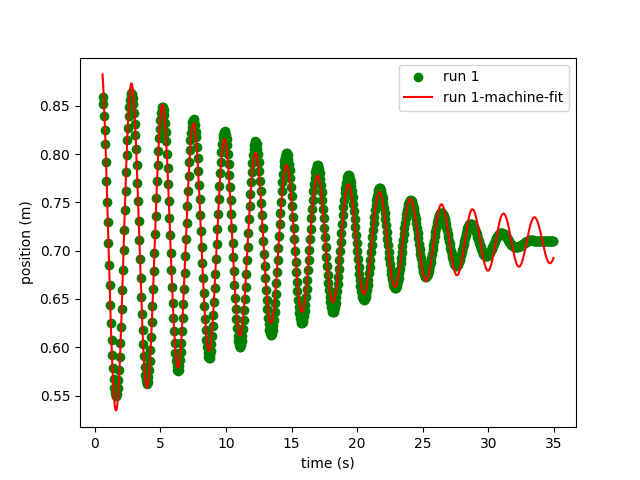
\includegraphics{Figure_0.png}\\
The model fits the curve relatively well until $t\to t_f$ where the error has built up the most and the fit begins to fail.
I guessed $x_0$ using the value of the data when $t=t_f$, $A$ by distance fromt the peak to $x_0$, $\beta$ was a complete guess
and $\omega_1$ and $\delta$ were slightly educated guess based on the shape of the graph. \\
$
x_0 = 0.71 \\
A = 0.177 \\
\beta = 0.05 \\
\omega_1 = 2.7 \\
\delta = 1.3 \\
$
and the machine adopted my guesses to \\
$
x_0 = 0.7099221 \\
A = -0.19411723 \\
\beta = 0.06157102 \\
\omega_1 = -2.6606827 \\
\delta = -4.34149397 \\
$
Which are generally close to mine but the machine seems to have decided that offsetting the curve by a lot fits
the data better. The uncertainty associated with each of these values is \\
$
x_{0u} = 0.000336763169790041 \\
A_u = 0.0016034606530748328 \\
\beta_u = 0.0007619444344572854 \\
\omega_{1u} = 0.000754079820004922 \\
\delta_u = 0.008039447229207356 \\
$
This run is the one which shows the greatest disagreement with the observed data. As I stated earlier the error piles up and
is most noticeable towards the end, this leads me to believe that the error originates from the fact that our model
does not incorporate friction as its effects would pile up and result in a greater velocity (change in position) than actually observed, which is 
what we see.

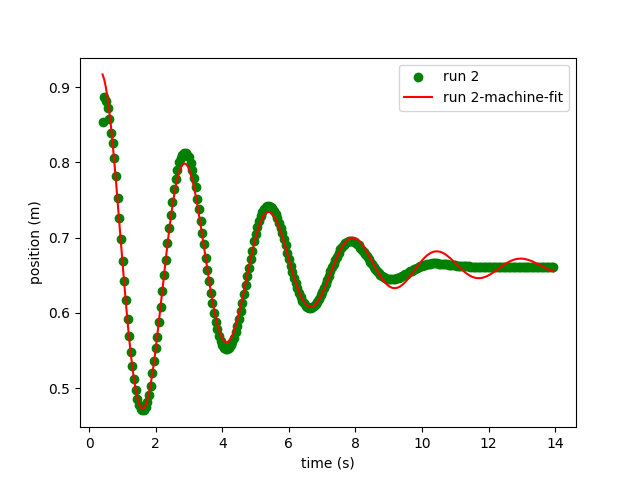
\includegraphics{Figure_1.png}\\
The model generally fits this curve much better, likely because this run is dampened more severly so friction is beaten out by the
dampening force. My guessing process was generally similar except I started from the parameters I guessed in run 1. \\
$
x_0 = 0.6606 \\
A = 0.2 \\
\beta = 0.05 \\
\omega_1 = 2.6 \\
\delta = 1.3 \\
$
and the machine adopted my guesses to \\
$
x_0 = 0.66118243 \\
A = 0.28286486 \\
\beta = 0.25038451 \\
\omega_1 = 2.48782223 \\
\delta = 0.9432566 \\
$
Which again are generally close to mine save, again, for the offset of phase and a pretty drastic change to beta that greatly improves the fit.\\
$
x_{0u} = 0.0005322378475141308 \\
A_u = 0.0033493873170781464 \\
\beta_u = 0.00386618733340337 \\
\omega_{1u} = 0.003997938882975206 \\
\delta_u = 0.012503337208939681 \\
$

\end{document}